% !TeX root = ../protokoll.tex
\part{Theorie}
\cref{fig:Einleitung/SchaltbildOperationsverstärker} zeigt das Schaltsymbol, 
welches für einen beliebigen Operationsverstärker gilt. Dieser hat einen 
"`Plus"'-Eingang ($+$) und einen "`Minus"'-Eingang ($-$) und einen Ausgang A.

\begin{figure}[H]
	\centering
	\begin{subfigure}[t]{0.3\linewidth}
		\centering
		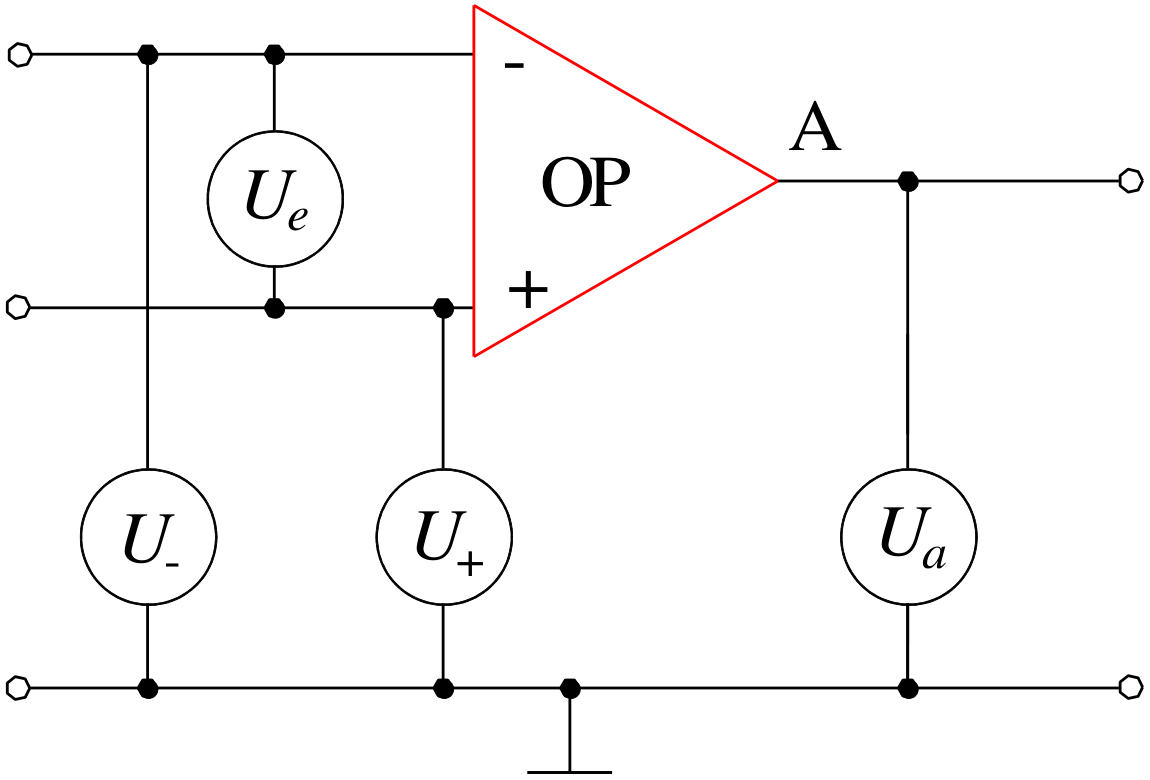
\includegraphics[width=\linewidth]{theorie/schaltbildOP}
		\caption{Schaltbild eines Operationsverstärkers ({\color{red} rot}), 
		entnommen aus \cite{script}}
		\label{fig:Einleitung/SchaltbildOperationsverstärker}
	\end{subfigure}
	\quad
	\begin{subfigure}[t]{0.2\linewidth}
		\centering
		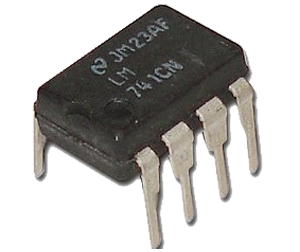
\includegraphics[width=\linewidth]{theorie/741}
		\caption{Abbild eines Operationsverstärkers vom Typ 741, entnommen aus 
		\cite{image741}}
		\label{fig:Einleitung/Operationsverstärker}
	\end{subfigure}
	\quad
	\begin{subfigure}[t]{0.3\linewidth}
		\centering
		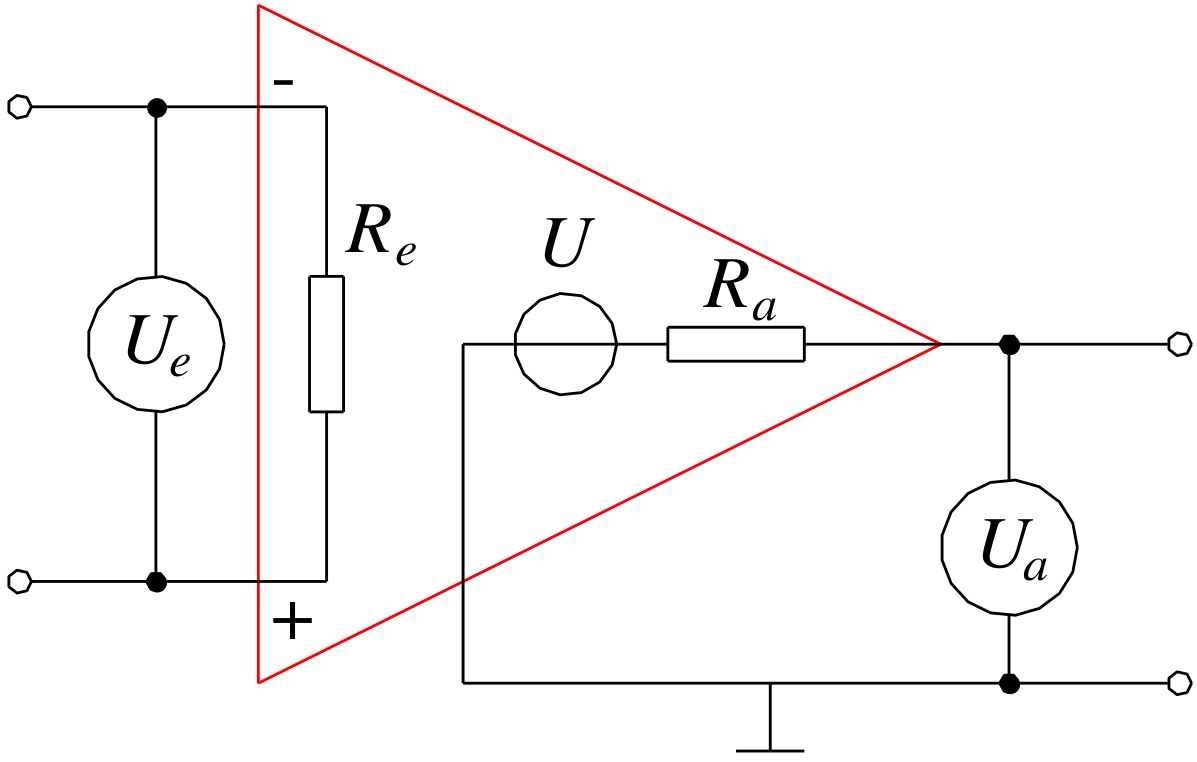
\includegraphics[width=\linewidth]{theorie/ersatzSchaltbildOP}
		\caption{Ersatzschaltbild eines Operationsverstärkers ({\color{red} 
		rot}) zur Definition es Eingangswiderstandes $R_e$ und des 
		Ausgangswiderstandes $R_a$, entnommen aus \cite{script}}
		\label{fig:Einleitung/ErsatzschaltbildOperationsverstärker}
	\end{subfigure}
	\caption{Darstellungen eines Operationsverstärkers}
\end{figure}

Der Operationsverstärker verstärkt hierbei die 
\textsl{Eingangsspannungsdifferenz} $U_e$:
\begin{equation}\label{eq:Eingangsspannungsdifferenz}
	U_e = U_+ - U_-
\end{equation}
mit dem \textsl{Leerlaufverstärkungsfaktor} $V_0 > 0$, womit für die 
\textsl{Ausgangsspannung} $U_a$ gilt:
\begin{equation}\label{eq:Ausgangsspannung}
	U_a = V_0 \cdot U_e = V_0 \cdot \left(U_e = U_+ - U_-\right).
\end{equation}
Wenn $U_- = \qty{0}{\V}$ folgt aus \cref{eq:Ausgangsspannung}:
\begin{equation}
	U_- = \qty{0}{\V} \quad \rightarrow \quad U_a = V_0 \cdot U_+
\end{equation}
In diesem Fall haben sowohl die Eingangs- als auch die Ausgangsspannung das 
gleiche Vorzeichen. Daher wird der "`Plus"'-Eingang als 
\textsl{nicht-invertierender} Eingang bezeichnet. Im Gegensatz dazu gilt für 
den Fall
\begin{equation}
	U_+ = \qty{0}{\V} \quad \rightarrow \quad U_a = -V_0 \cdot U_-
\end{equation}
dass die Eingangsspannung $U_-$ und die Ausgangsspannung $U_a$ entgegengesetzte 
Vorzeichen haben. Daher wird der "`Minus"'-Eingang eines Operationsverstärkers 
auch \textsl{invertierender} Eingang genannt.

Ein idealer Operationsverstärker hat einen unendlich großen 
Leerlaufverstärkungsfaktor $V_0 \rightarrow \infty$ (vgl. 
\cref{fig:Einleitung/ErsatzschaltbildOperationsverstärker}), einen unendlich 
großen 
Eingangswiderstand $R_e \rightarrow \infty$ (vgl. 
\cref{fig:Einleitung/ErsatzschaltbildOperationsverstärker}), einen 
verschwindend kleinen Ausgangswiderstand $R_a \rightarrow 0$ (vgl. 
\cref{fig:Einleitung/ErsatzschaltbildOperationsverstärker}) und eine 
frequenzunabhängige Verstärkung. Ein realer Operationsverstärker weicht 
natürlich von diesem Idealvorstellungen ab: die Widerstände sind weder 
unendlich groß noch verschwindend klein, auch der Leerlaufverstärkungsfaktor 
hat seine Grenze und die Verstärkung findet frequenzabhängig statt.

Für die folgenden Überlegungen wird jedoch trotzdem der Operationsverstärker 
als eine "`Black Box"' angenommen und mit den idealen Eigenschaften betrachtet.

\section{Mit- und Gegenkopplung}
Aufgrund des großen Leerlaufverstärkungsfaktors $V_0$ ist der 
Operationsverstärker nicht ohne äußere Beschaltung nutzbar, da nach
\cref{eq:Ausgangsspannung} bereits kleine Eingangsspannungsdifferenzen $U_e$ im
\unit{\micro\V}- bis \unit{\mV}-Bereich zum Erreichen der maximalen 
Ausgangsspannung führen. Die maximale Ausgangsspannung ist hierbei abhängig von
der eingesetzten Betriebsspannung, welche typischerweise $\pm \qty{12}{\V}$
beträgt. Aufgrund dieses Verhaltens wird ein teil der Ausgangsspannung
auf den invertierenden Eingang des Operationsverstärkers zurückgekoppelt. Dies
hat zur Folge, dass eine Änderung der Ausgangsspannung einer Änderung der
Eingangsspannungsdifferenz $U_e$ entgegenwirkt. Daher auch der Name 
"`Gegenkopplung"'

Würde nun umgekehrt eine Änderung der Ausgangsspannung auch eine gleichsinnige
Änderung des Eingangsspannungsdifferenz bewirken, da ein Teil der 
Ausgangsspannung auf den nicht-invertierenden Eingang zurückgekoppelt wird, so
wäre der Operationsverstärker Mitgekoppelt und der Operationsverstärker Würde
übersteuern.

In den folgenden Abschnitten werden verschiedene Schaltungen eines 
Operationsverstärkers betrachtet.

\section{Beschaltungen eines Operationsverstärkers}
\subsection{Invertierender Verstärker}
Für einen invertierenden Verstärker wird eine gegengekoppelte Beschaltung des
Operationsverstärkers gemäß \cref{fig:Theorie/invertierenderVerstärker} 
betrachtet.

\begin{figure}[H]
	\centering
	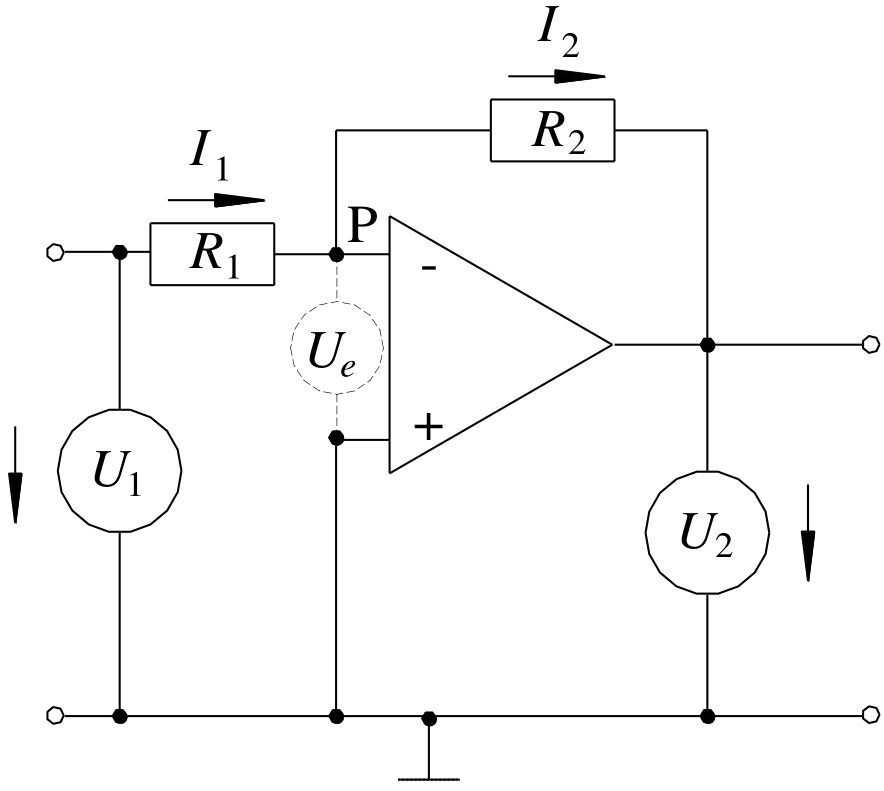
\includegraphics[width=0.3\linewidth]{theorie/schaltbild-invertierenderVerstärker}
	\caption{Invertierender Verstärker. Alle Spannungen werden auf das 
	Massepotential bezogen. Die Klemmenspannung $U_1$ zwischen den 
	Eingangsbuchsen (offene Kreise links) angelegt. Die Ausgangsspannung wird
	ziwschen den Ausgangsbuchsen (offene Kreise rechts) abgegriffen, entommen
	aus \cite{script}}
	\label{fig:Theorie/invertierenderVerstärker}
\end{figure}

Die zu verstärkende Klemmenspannung $U_1$ wird über den Widerstand $R_1$ auf den
invertierenden Eingang des Operationsverstärkers gegeben, auf den gleichzeitig
über den Widerstand $R_2$ die Ausgangsspannung $U_2$ zurückgekoppelt wird.

Aufgrund des hohen Eingangswiderstandes es Operationsverstärkers fließt
praktisch kein Strom in den Operationsverstärker. Somit gilt nach der 
Knotenregel für den Punkt P:
\begin{equation}
	I_1 - I_2 = 0
\end{equation}
woraus folgt, dass:
\begin{equation}\label{eq:Stromstärkengleichgewicht}
	I_1 = I_2 := I
\end{equation}

Wird diese Schaltung nun im Zeitlupentempo betrachtet, so sind alle Spannungen
anfangs gleich null. Wird nun eine positive Klemmenspannung $U_1$ angelegt, so
steigt die Eingangsspannung $U_-$, da $U_2$ in diesem Momnent noch null ist.
Da $U_+$ der Massekontakt ist und somit konstant null ist, gilt nach
\cref{eq:Eingangsspannungsdifferenz}:
\begin{equation}
	U_e = - U_-
\end{equation}
Diese Spannung wird nun mit dem Faktor $V_e$ verstärkt und erzeugt dadurch eine
Ausgangsspannung $U_2$ (vgl. \cref{eq:Ausgangsspannung}). Damit ist $U_2$ 
negativ und verringert über die Rückkopplung über $R_2$ die Spannung $U_-$. Dies
verringert nun die Ausgangsspannung, was wiederum über die Rückkopplung die
Spannung $U_-$ verringert, bis die Eingangsspannungsdifferenz $U_e$ einen Wert
von etwa \qty{0}{\V} erreicht. Dadruch hat der nicht-invertierende Eingang 
nahezu das gleiche Potential. Wird dieses nun auf die Masse bezogen, gilt:
\begin{equation}
	U_- \approx U_+ = \qty{0}{\V}
\end{equation}
Somit fällt praktisch die Klemmenspannung $U_1$ vollständig über den Widerstand
$R_1$ ab und die gesamte Ausgangsspannung über $R_2$ ab, sodass laut der
Maschenregel und \cref{eq:Stromstärkengleichgewicht} gilt (Vorzeichen nach 
\cref{fig:Theorie/invertierenderVerstärker}):
\begin{equation}\label{eq:uri1}
	U_1 = R_1 \cdot I
\end{equation}
\begin{equation}\label{eq:uri2}
	U_2 = - R_2 \cdot I
\end{equation}

Werden nun \cref{eq:uri1,eq:uri2} nach $I$ aufgelöst und gleichgesetzt ergibt
sich:
\begin{equation}
	\dfrac{U_1}{R_1} = -\dfrac{U_2}{R_2}
\end{equation}
und damit:
\begin{equation}
	U_2 = - U_1 \dfrac{R_2}{R_1}
\end{equation}
Damit gilt für das Verhältnis der Ausgangsspannung zur Klemmenspannung $V$:
\begin{equation}\label{eq:Klemmenspannung}
	V = \dfrac{U_2}{U_1} = - \dfrac{R_2}{R_1}
\end{equation}

Für Wechselspannungen ist $V$ als das Verhältnis der Spannungsamplituden 
definiert
\begin{equation}\label{eq:KlemmenspannungAC}
	V = \dfrac{U_{2,0}}{U_{1,0}} = - \dfrac{R_2}{R_1}
\end{equation}

$V$ wird auch die "`Klemmenverstärkung"' genannt.
\newpage
\subsection{Frequenzgang, Grenzfrequenz und Verstärkungs-Bandbreite Produkt}
Nach den \cref{eq:Klemmenspannung,eq:KlemmenspannungAC} ist der 
Verstärkungsfaktor $V$ ausschließlich durch das Verhältnis von $R_1$ und $R_2$
angegeben. Jedoch wurde hier nur ein idealer Zustand betrachtet und in der 
Realität findet die Verstärkung frequenzabhängig statt. Der Verlauf des
realen Verstärkungsfaktors $V_r$ nennt sich "`Frequenzgang"' oder auch
"`Amplitudenübertragungsfunktion"'

Der Frequenzgang wird druch folgende Gleichung gegeben
\begin{equation}\label{eq:Frequenzgang}
	V_r(f) = V_s \dfrac{1}{
		\sqrt{1 + \left(
			\dfrac{f}{f_g}
		\right)^2}
	}
\end{equation}
mit der Sollverstärkung $V_s$
\begin{equation}\label{eq:Sollverstärkung}
	V_s = - \dfrac{R_2}{R_1}
\end{equation}
und der Grenzfrequenz $f_g$, die erreicht ist, wenn folgendes gilt:
\begin{equation}
	V_r = \dfrac{V_s}{\sqrt{2}}
\end{equation}

Wird nun die Grenzfrequenz überschritten, so sinkt der reelle Verstärkungsfaktor
um den selben Faktor um den die Frequenz $f$ zunimmt. Sinkt der Wert von $V_r$
auf 1, so ist die Transitfrequenz $f_T$ erreicht.

\subsection{Nicht-invertierender Verstärker}
Um einen nicht-invertierenden Verstärker aufzubauen reicht es nicht, einfach
"`+"' und "`-"' zu vertauschen, da somit eine Mittkopplung entstehen würde. Die
Schaltung aus \cref{fig:Theorie/invertierenderVerstärker} muss umgebaut werden
zu \cref{fig:Theorie/nicht-invertierenderVerstärker}.
\begin{figure}[H]
	\centering
	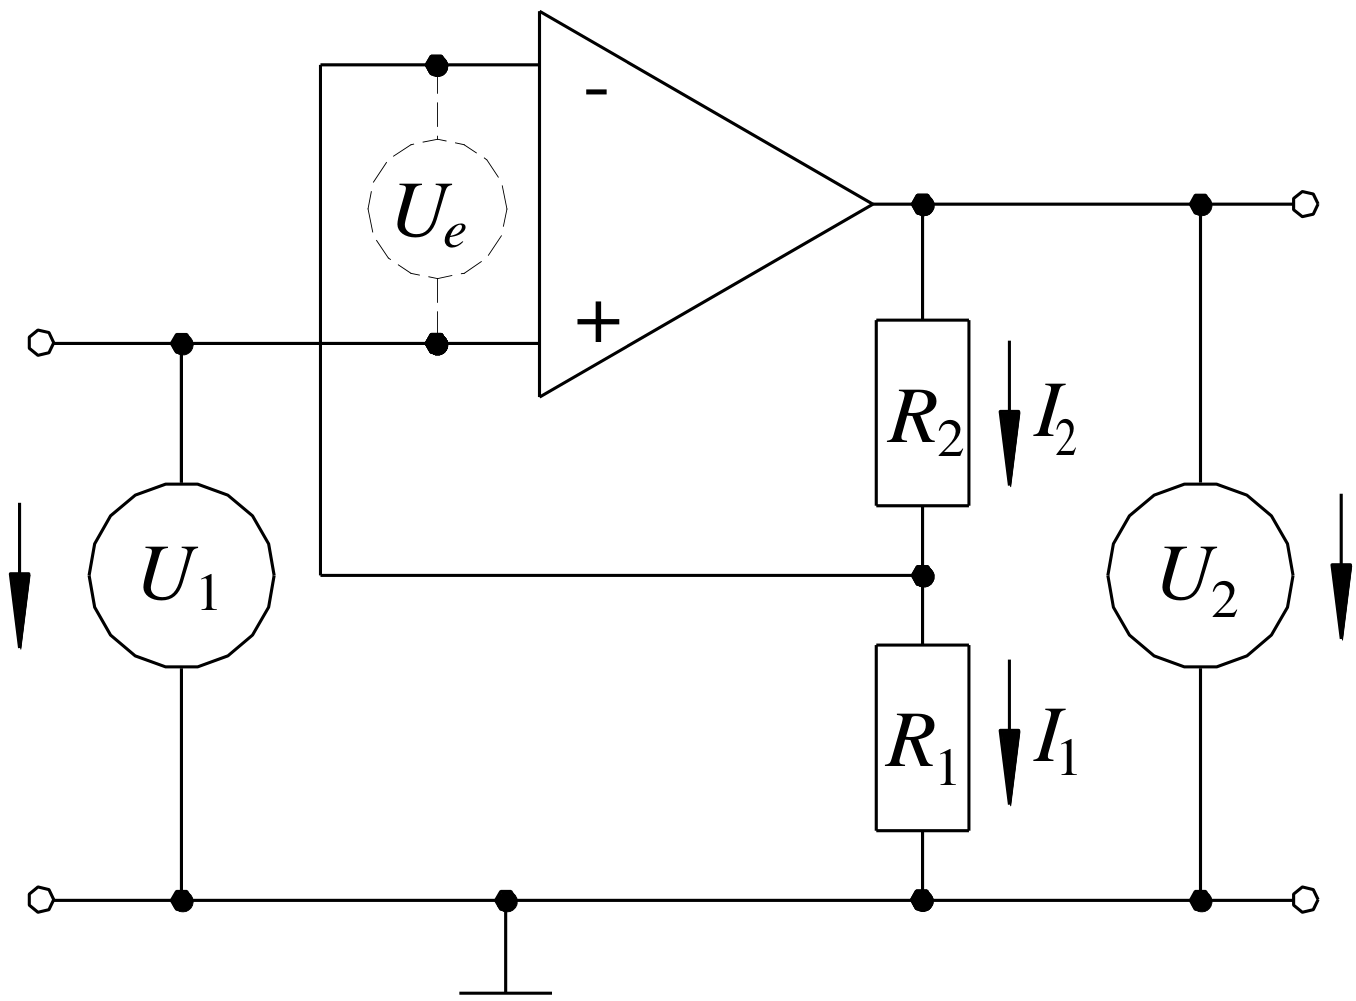
\includegraphics[width=0.3\linewidth]{theorie/schaltbild-nicht-invertierenderVerstärker}
	\caption{nicht-invertierender Verstärker, entommen
	aus \cite{script}}
	\label{fig:Theorie/nicht-invertierenderVerstärker}
\end{figure}

Die Klemmenverstärkung beträgt in diesem Fall
\begin{equation}
	V = \dfrac{U_2}{U_1} = 1 + \dfrac{R_2}{R_1}
\end{equation}

\subsection{Integrator (invertierend)}
Mithilfe einer Gegenkopplung wie in \cref{fig:Theorie/integrator} lässt sich
ein Spannungssignal integrieren. Hierbei wird erneut die Knotenregel auf den
Punkt P angewendet, sodass in den Operationsverstärker praktisch keinen Strom
fließt, sodass gilt:
\begin{equation}
	I_1 - I_2 = 0
\end{equation}
und damit auch
\begin{equation}
	I_1 = I_2 := I
\end{equation}

\begin{figure}[H]
	\centering
	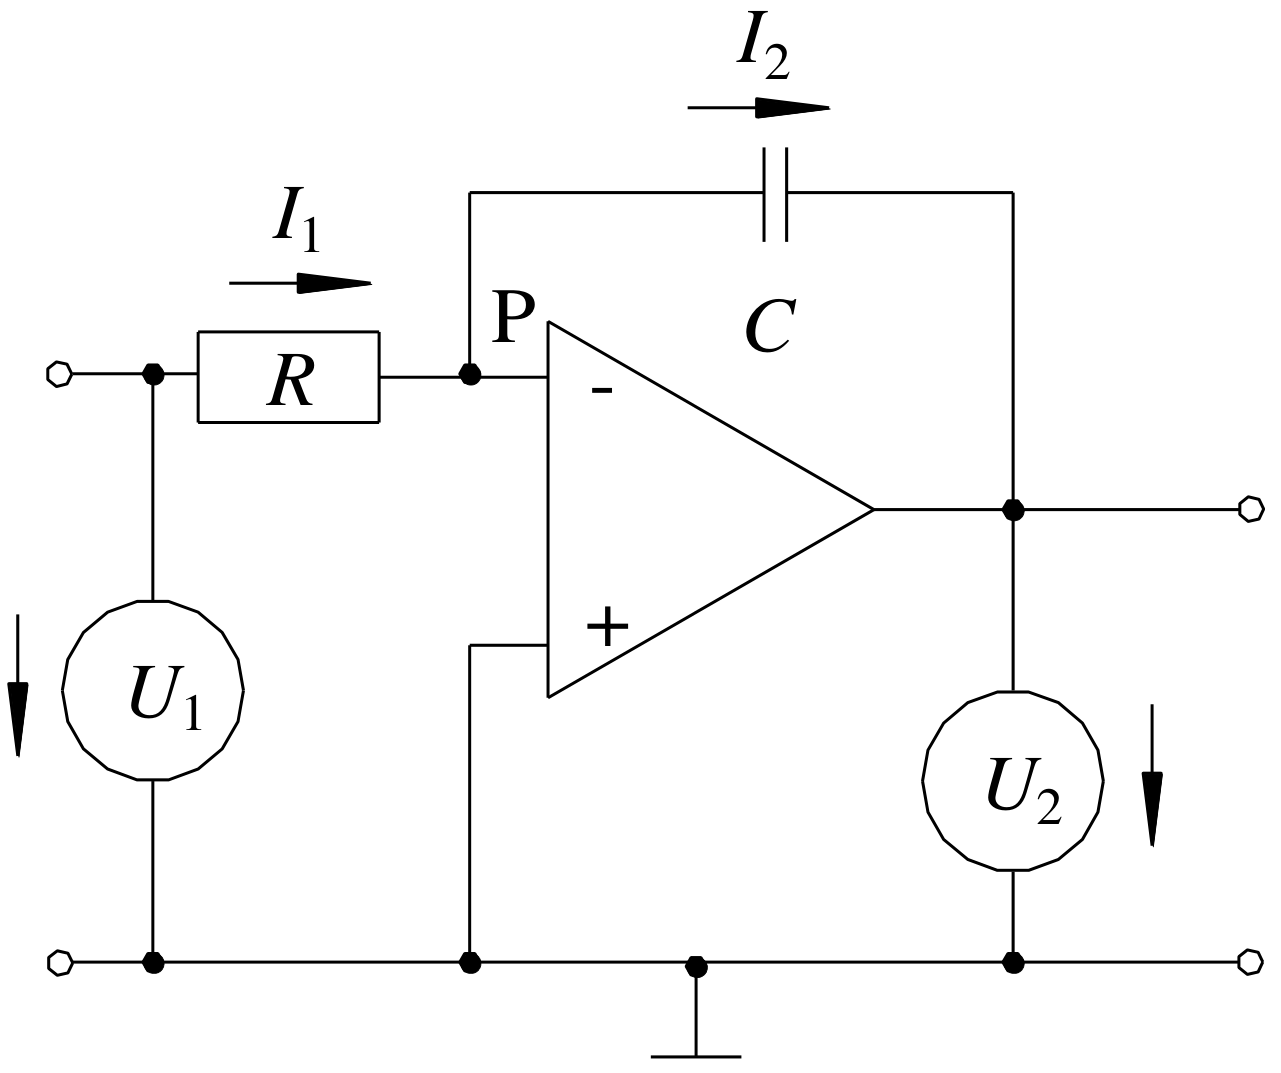
\includegraphics[width=0.3\linewidth]{theorie/schaltbild-integrator}
	\caption{Schaltbild eines Integrators, entommen
	aus \cite{script}}
	\label{fig:Theorie/integrator}
\end{figure}

Für den Strom, welcher durch den Widerstand $R$ fließt, gilt laut der 
Maschenregel und der Gegenkopplung:
\begin{equation}\label{eq:Integrator/Widerstand}
	I = \dfrac{U_1}{R}
\end{equation}
und für den Strom durch den Kondensator $C$
\begin{equation}\label{eq:Integrator/Kondensator}
	I = -C \diff{U_2}{t}
\end{equation}
Werden nun die \cref{eq:Integrator/Widerstand,eq:Integrator/Kondensator} 
gleichgesetzt, so ergibt sich:
\begin{equation}
	\diff{U_2}{t} = - \dfrac{1}{RC} U_1
\end{equation}
Integration über $t$ liefert nun die Ausgangsspannung $U_2$:
\begin{equation}\label{eq:Integrator/Ausgangsspannung}
	U_2 = - \dfrac{1}{RC} \int U_1 \mathrm{d}t
\end{equation}

Nun wird der Spezialfall einer sinusförmigen Klemmenspannung mit der Frequenz
$f$, der daraus berechenbaren Kreisfrequenz $\omega = 2 \pi f$ und der Amplitude
$U_{1,0}$, betrachtet. Somit ergibt sich für die Klemmenspannung
\begin{equation}
	U_1 = U_{1,0} \sin \omega t
\end{equation}

Für diesen Fall gilt für die Ausgangsspannung nach 
\cref{eq:Integrator/Ausgangsspannung}:
\begin{align}
	\begin{split}
		U_2 &= - \dfrac{1}{RC} \int U_{1,0} \sin \omega t \mathrm{d}t \\
		&= \dfrac{U_{1,0}}{\omega R C} \cos \omega t \\
		&:= U_{2,0} \cos \omega t
	\end{split}
\end{align}
mit $U_{2,0} = \dfrac{U_{1,0}}{\omega R C}$

Für die Klemmenverstärkung gilt in diesem Fall:
\begin{equation}\label{eq:Integrator/AC-Klemmenverstärkung}
	V = \dfrac{U_{2,0}}{U_{1,0}} = \dfrac{1}{\omega R C}
\end{equation}

Das Verhalten eines Integrators bei hohen Frequenzen entspricht nach
\cref{eq:Integrator/AC-Klemmenverstärkung} dem Verhalten eines
Tiefpasses.

Wird zusätzlich zu dem Verstärkungsfaktor $V$ die zeitabhänigigen Teile der
Klemen- und Ausgangsspannung betrachtet, so beträgt deren Phasenverschiebung
konstant:
\begin{equation}
	\left| \Delta \varphi \right| = \qty{90}{\degree}
\end{equation}

\subsection{Differentiator (invertierend)}
Wird eine Schaltung nach \cref{fig:Theorie/Differentiator} benutzt, so können
Spannungssignale differenziert werden. Nach analogen Überlegungen wie im 
vorherigen Kapitel ergibt sich folgende Beziehung:
\begin{equation}
	U_2 = - R C \diff{U_1}{t}
\end{equation}

\begin{figure}[H]
	\centering
	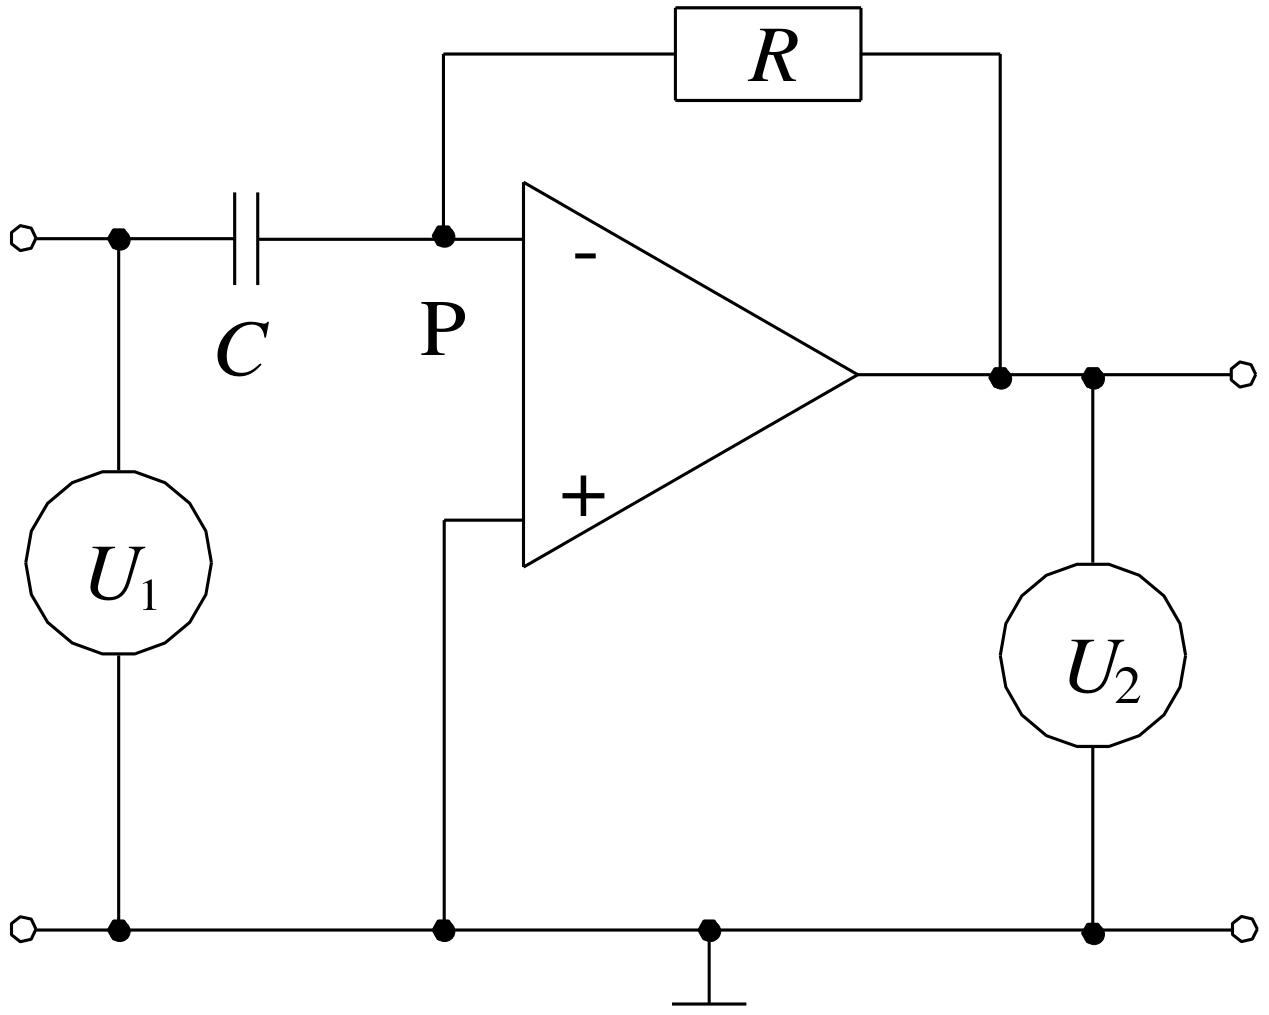
\includegraphics[width=0.3\linewidth]{theorie/schaltbild-differentiator}
	\caption{Schaltbild eines Differentiators, entommen
	aus \cite{script}}
	\label{fig:Theorie/Differentiator}
\end{figure}

Wird auch hier nun mit einer sinusförmigen Wechselspannungen gearbeitet, so
gilt für die Klemmenverstärkung:
\begin{equation}
	V = \omega R C
\end{equation}
Somit verhält sich ein Differentiator wie ein Hochpass und verstärkt hohe 
Frequenzen mehr als niedrige Frequenzen. Des Weiteren beträgt auch hier die
Phasenverschiebung konstant:
\begin{equation}
	\left| \Delta \varphi \right| = \qty{90}{\degree}
\end{equation}

\subsection{Impedanzwandler}
Impedanzwandler (vgl. \cref{fig:Theorie/Impedanzwandler}) werden benutzt um
Signalquellen mit einem hohen Innenwiderstand and Schaltungen mit niedrigem
Eingangswiderstand anzupassen. Hierbei wird der Ausgang der Signalquelle mit
seiner Spannung $U_1$ direkt an den "`+"'-eingang des Operationsverstärkers
verbunden. Der Ausgang des Operationsverstärkers wird hierbei auf den 
"`-"'-Eingang zurückgekoppelt. Am Ausgang liegt somit die selbe Spannung an und
der kleine Ausgangswiderstand erlaubt nun den Anschluss an eine Schaltung mit
einem niedrigen Eingangswiderstand.

\begin{figure}[H]
	\centering
	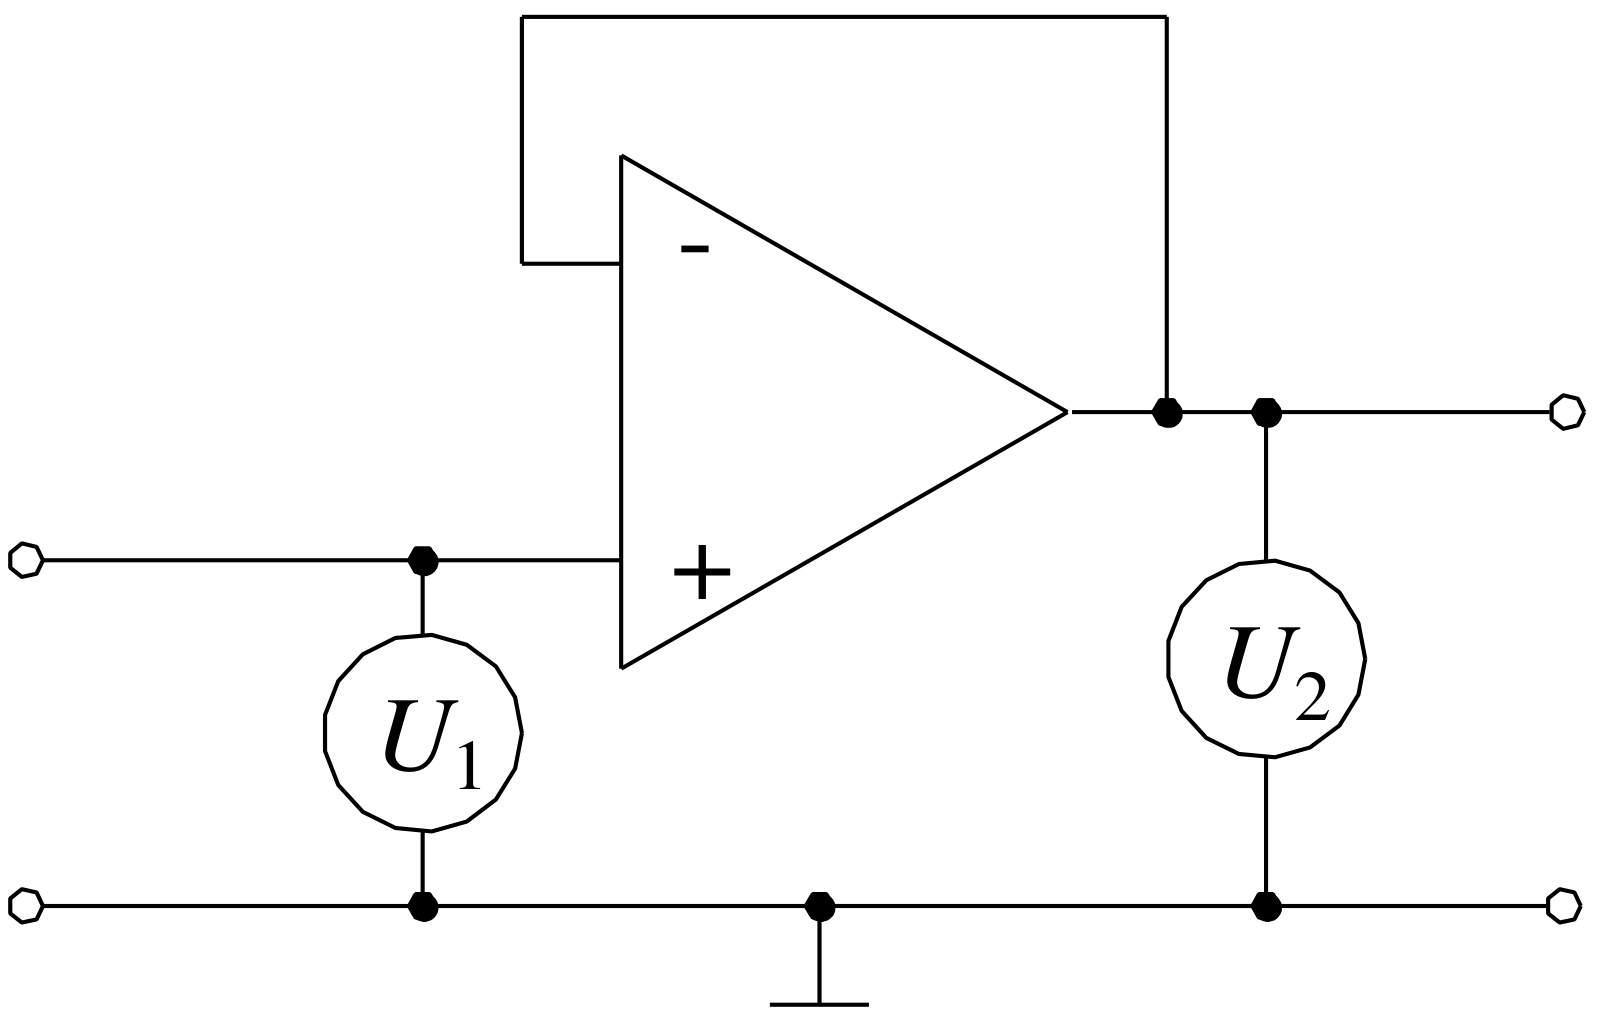
\includegraphics[width=0.3\linewidth]{theorie/schaltbild-impedanzwandler}
	\caption{Schaltbild eines Impedanzwandlers, entommen
	aus \cite{script}}
	\label{fig:Theorie/Impedanzwandler}
\end{figure}

\subsection{Transimpedanzverstärker, Strom-Spannungs-Wandler}
Ein Transimpedanzverstärker (vgl. \cref{fig:Theorie/Transimpedanzverstärker})
wird verwendet, um einen Eingangsstrom $I_1$ in eine dazu proportionale 
Ausgangsspannung $U_2$ zu wandeln. Aus den selben Überlegungen wie bei den
bereits beschriebenen Beschaltungen folgt:
\begin{equation}
	I_1 = I_2 := I
\end{equation}
und
\begin{equation}
	U_2 = - R I
\end{equation}

Als Transimpedanz $Z$ wird hierbei  der Betrag des Quotienten aus 
Ausgangsspannung und Eingangsstrom bezeichnet:
\begin{equation}
	Z = \left| \dfrac{U_2}{I} \right| = R
\end{equation}
und bestimmt den Proportinalitätsfaktor zwischen Eingangsstrom und 
Ausgangsspannung. Somit können mit Hilfe von großen Widerständen kleine 
Ströme in große Spannungen gewandelt werden. Dieses Verfahren wird 
beispielsweise bei der Messung des Fotostroms einer Fotodiode benutzt.

\begin{figure}[H]
	\centering
	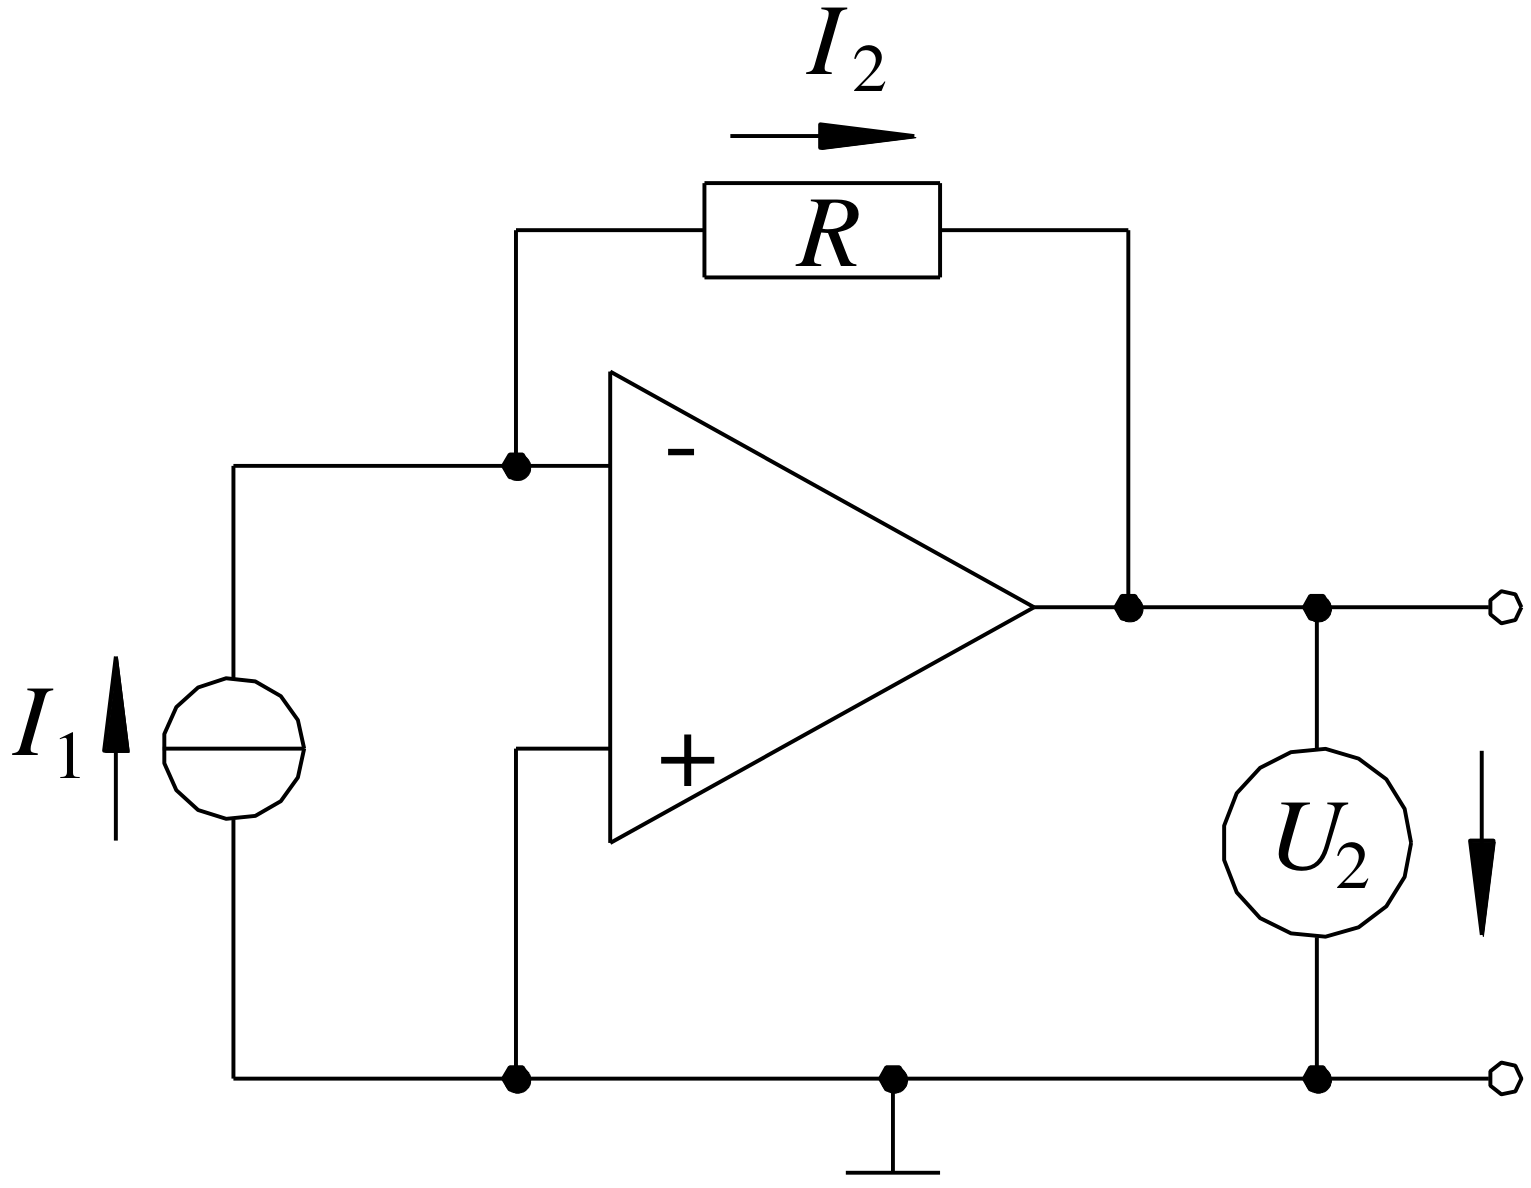
\includegraphics[width=0.3\linewidth]{theorie/schaltbild-transimpedanzverstärker}
	\caption{Schaltbild eines Transimpedanzverstärker, entommen
	aus \cite{script}}
	\label{fig:Theorie/Transimpedanzverstärker}
\end{figure}